\documentclass{scrartcl}
\usepackage[utf8]{inputenc}
\usepackage[english]{babel} % Trennung nach der neuen deutschen Rechtschreibung
\usepackage[utf8]{inputenc}
\usepackage[T1]{fontenc}
\usepackage{lmodern}
\usepackage{subcaption}
\usepackage{chemformula}
\usepackage{placeins}
\usepackage{multirow}
\usepackage{enumitem}
\usepackage{amssymb}
\usepackage{amsmath} % Erweiterte Mathematik-Umgebung
\usepackage{amsfonts} % zusätzliche Mathematik-Schrifttypen (v.a. \mathbb für Mengen)
\usepackage{ulem}
\usepackage{amsthm}
\usepackage{graphics}%soll beim Graphiken einfügen hilfreich sein
\usepackage{graphicx}
\usepackage{wrapfig}%lässt Textumflossene Bildeinbindung zu
\usepackage{epstopdf}%soll eps in pdf umwandeln
\usepackage{placeins}
\usepackage{amsthm}
\usepackage{subcaption}
\usepackage{wrapfig}
\usepackage{float}
\usepackage{hyperref}
\usepackage{ragged2e}

\usepackage[a4paper, portrait, margin=2.5cm]{geometry}

\setlength\parindent{0pt}

\begin{document}

\begin{titlepage}
    \begin{center}
        \vspace*{1cm}
        \Huge
        \textbf{Magnetic properties of atoms}
        
        \vspace{0.5cm}
        \LARGE
        \textit{PART I: Induction and electron spin resonance}
        
        \vspace{0.5cm}
        \LARGE
        Advanced Lab Course
        
        \vspace{1.5cm}
        \textbf{Louis-Hendrik Barboutie (020157041C), Frederik Ehl (0201719742) and Florence Schmerber (0201845640)}
        
        \vspace{1cm}
        Supervisor: Jörg Baller
        \vfill
        

        
\includegraphics[width=0.4\textwidth]{logo_uni.jpg}
        
        \Large
        $28^{\underline{\text{th}}}$ March 2022
    \end{center}
\end{titlepage}

\section{Experimental setup \& procedure}

\subsection{Induction}
There are two coils at our disposition; only one is powered. We can modify the frequency of the current going through the coil. When the second coil is approached to the first one, and they are properly aligned, a current is induced in it. This phenomenon can be directly measured via the absorbed voltage in the first coil and the induced voltage in the second coil. There is also a capacitor inside the circuit connected to the second coil, whose capacitance we can modify. The induced voltage is measured with the voltmeter, whereas the absorbed voltage is measured with an oscilloscope. The actual setup can be seen in fig.~\ref{fig:setup_induction}. The goal of this experiment is to study the induction phenomenon.


\subsection{Electron spin resonance (ESR)}
The setup consist of two Helmholtz coils with constant magnetic field $B_0$. Between the coils, a sample containing the substance DDPH is placed inside a small coil, with magnetic field $B$, which is connected to a high frequency generator (see figure \ref{fig:setup_ESR}.) The frequency as well as the current can be modified.\\
We vary the frequency in steps of 3 MHz. Then we adjust the oscilloscope so that the signal of the Helmholtz coils and the one of the resonance coil are equidistant to each other, and only then the applied current is recorded. We do the same procedure for coils of different sizes, so that we get a full range between 30 and 100 MHz.\\
In order to determine the Landé factor $g_s$, we plot the frequency as a function of the magnetic field of the Helmhotz coils. This field can be calculated by using the following formula:
\begin{equation}
    B = \mu_0 \left( \frac{4}{5} \right)^\frac{3}{2}\frac{n}{r}I
    \label{equation_B}
\end{equation}
with I being the current, n the amount of loops of the coils and r the radius of the coils. In our case this is equivalent to :
\begin{equation}
    B = 4.23 \cdot I \ \text{mT}
\end{equation}
The small coil produces a small solenoid field which allows us slightly modify the total field in the sample. We can change this field and measure the absorbed voltage of the coil, and when the peaks are equidistant the absorbed voltage reaches its maximum.
\begin{figure}[H]
     \centering
     \begin{subfigure}[b]{0.45\textwidth}
         \centering
         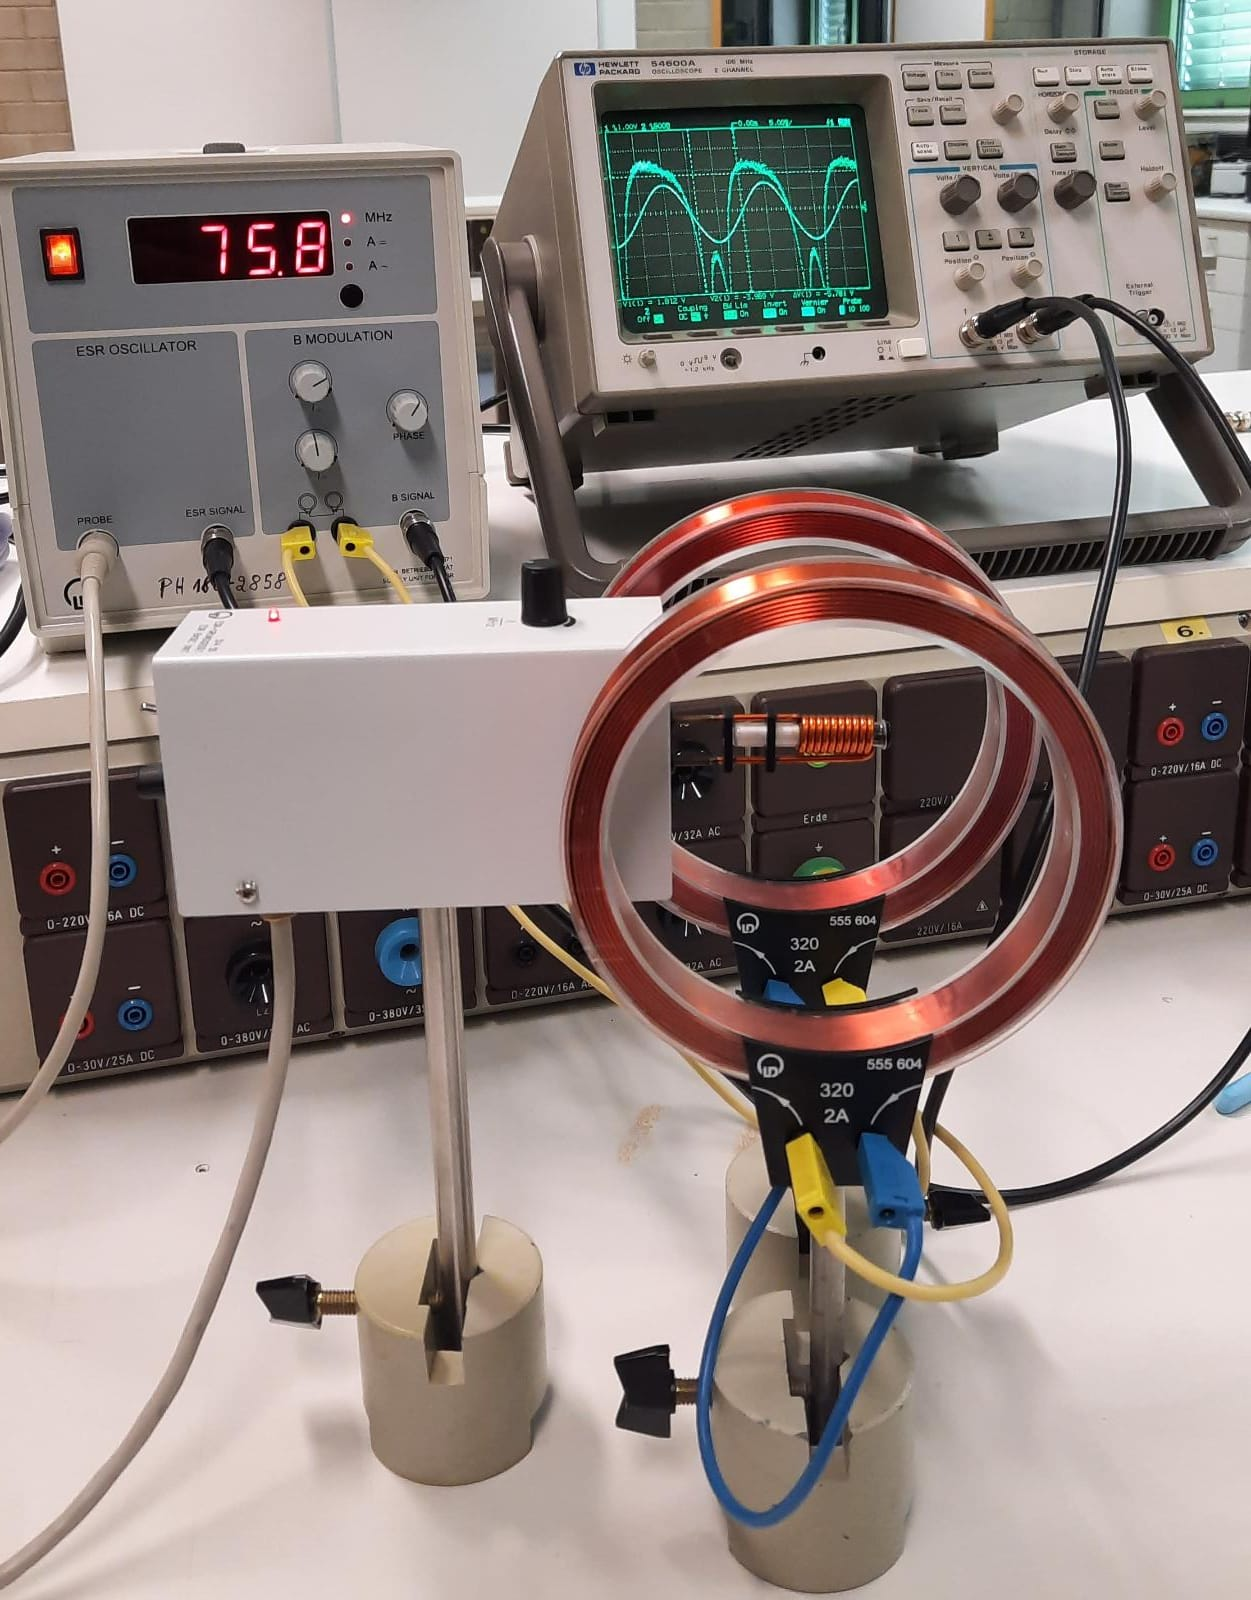
\includegraphics[width=0.7\textwidth]{bilder/1652518772134.jpg}
         \caption{Setup for ESR Experiment}
         \label{fig:setup_ESR}
     \end{subfigure}
     \hfill
     \begin{subfigure}[b]{0.45\textwidth}
         \centering
         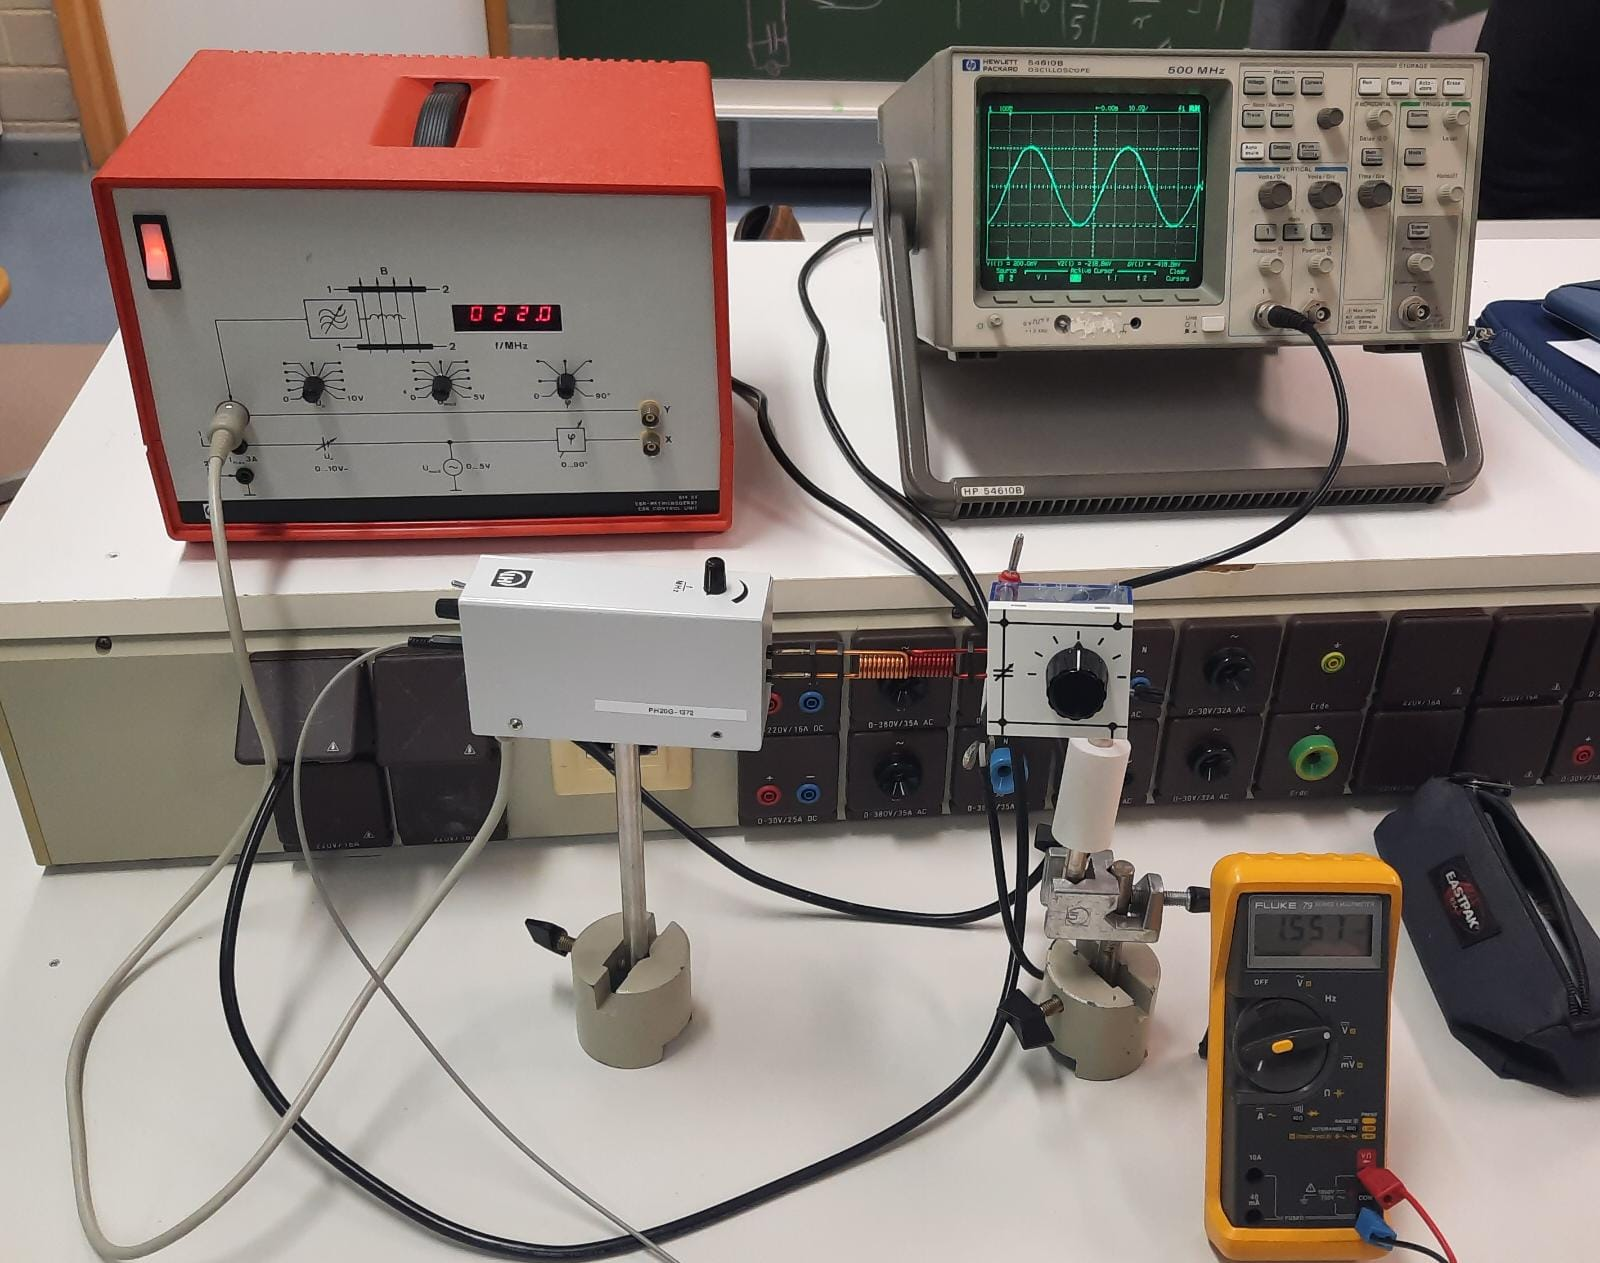
\includegraphics[width=\textwidth]{bilder/1652518991486.jpg}
         \caption{Setup for Induction Experiment}
         \label{fig:setup_induction}
     \end{subfigure}
     \caption{Setups for the two experiments}
     \label{fig:setups}
\end{figure}


%fluctuation of the voltage
%change the frequency and record the current
\section{Results and discussion}

\subsection{Induction}
The study of the influence of the frequency and capacitor yielded the graphs from fig.~\ref{fig:VoltageCap1}, fig.~\ref{fig:VoltageCap2} and fig.~\ref{fig:VoltageCap3}. The capacity of the powered coil is increasing in the following order: setting 3 < setting 1 < setting 2.

In fig.~\ref{fig:VoltageCap1} and fig.~\ref{fig:VoltageCap2}, the peak of induced voltage is reached for the same frequency as for the peak of absorbed voltage. While the absorbed voltage has a tendency to steadily increase, it suddenly drops, as the induced voltage is about to reach its maximum. This phenomenon isn't observable for the third capacitor setting in fig.~\ref{fig:VoltageCap3}, as the maximum of induced voltage lies in the frequency region below 22 MHz. The experimental setup did not have the possibility to go into such frequency ranges. 

Since the induced and absorbed voltages have a dependency on frequency, it might be possible however to observe the same peaks for integer multiples of the frequency. A limiting factor in this case is the absorbed voltage, which is finite at some point. 

\begin{figure}[!ht]
    \centering
    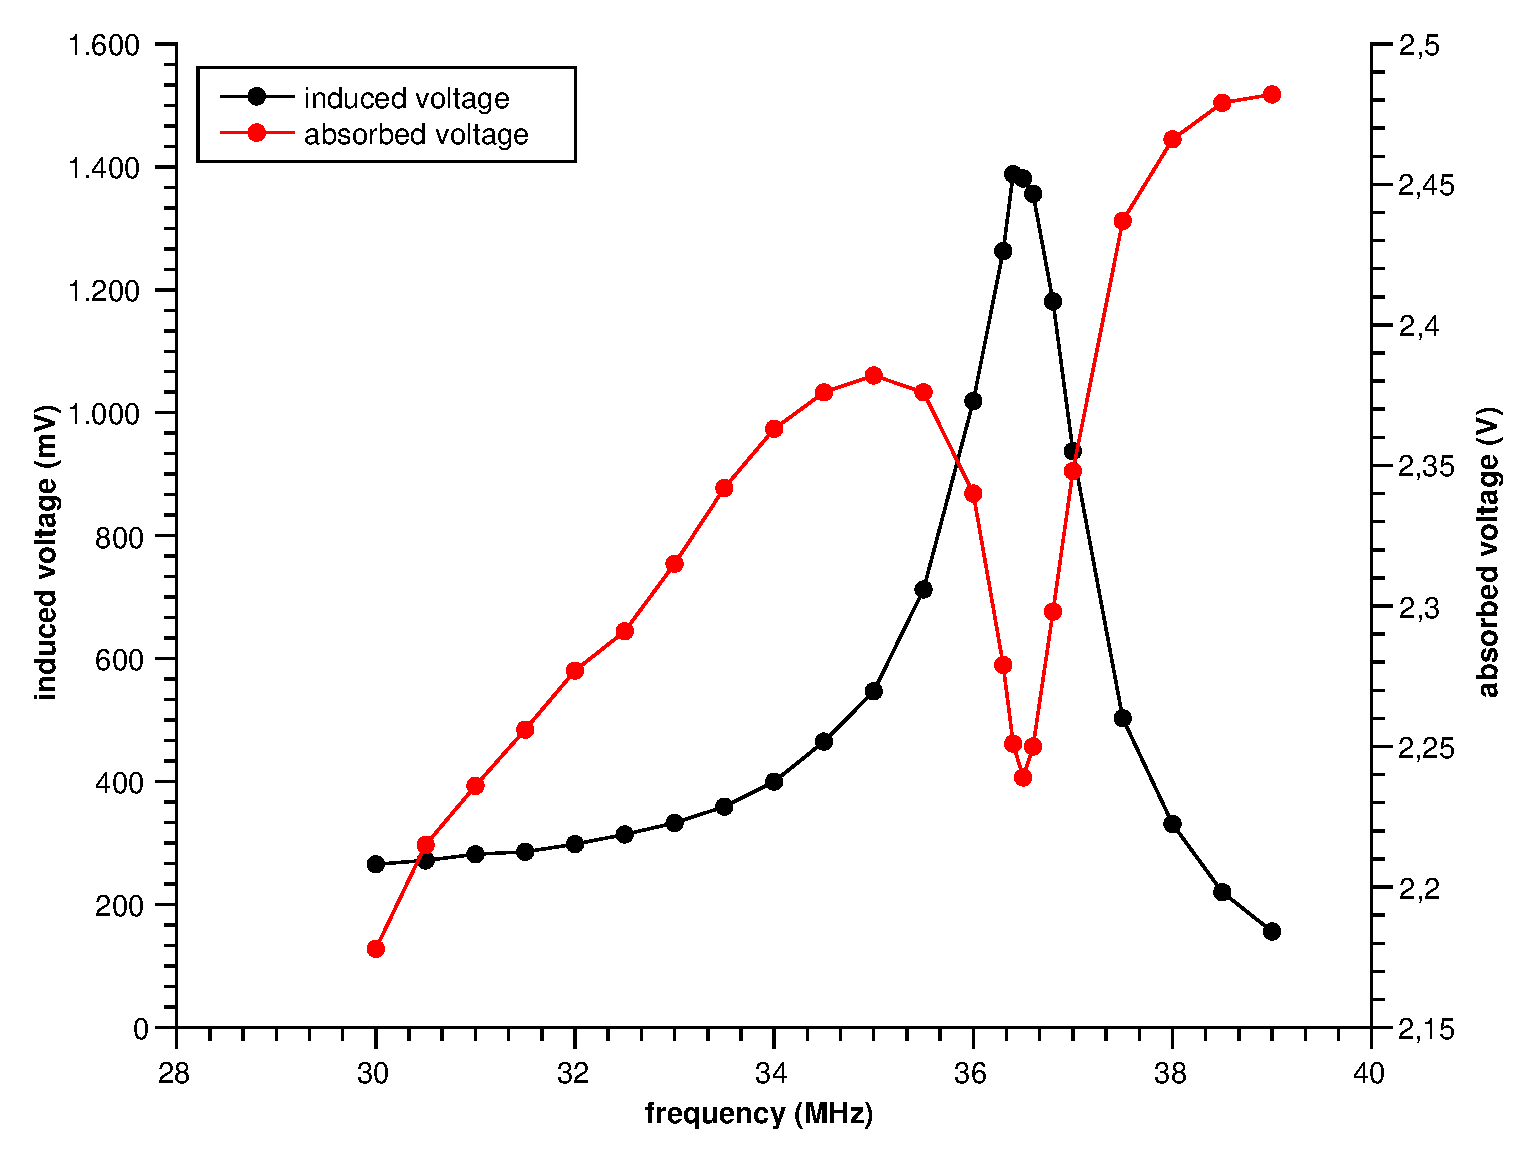
\includegraphics[width=0.8\textwidth]{Capacitor1.eps}
    \caption{Induced and absorbed voltages for capacitor setting 1}
    \label{fig:VoltageCap1}
\end{figure}

\begin{figure}[!ht]
    \centering    
    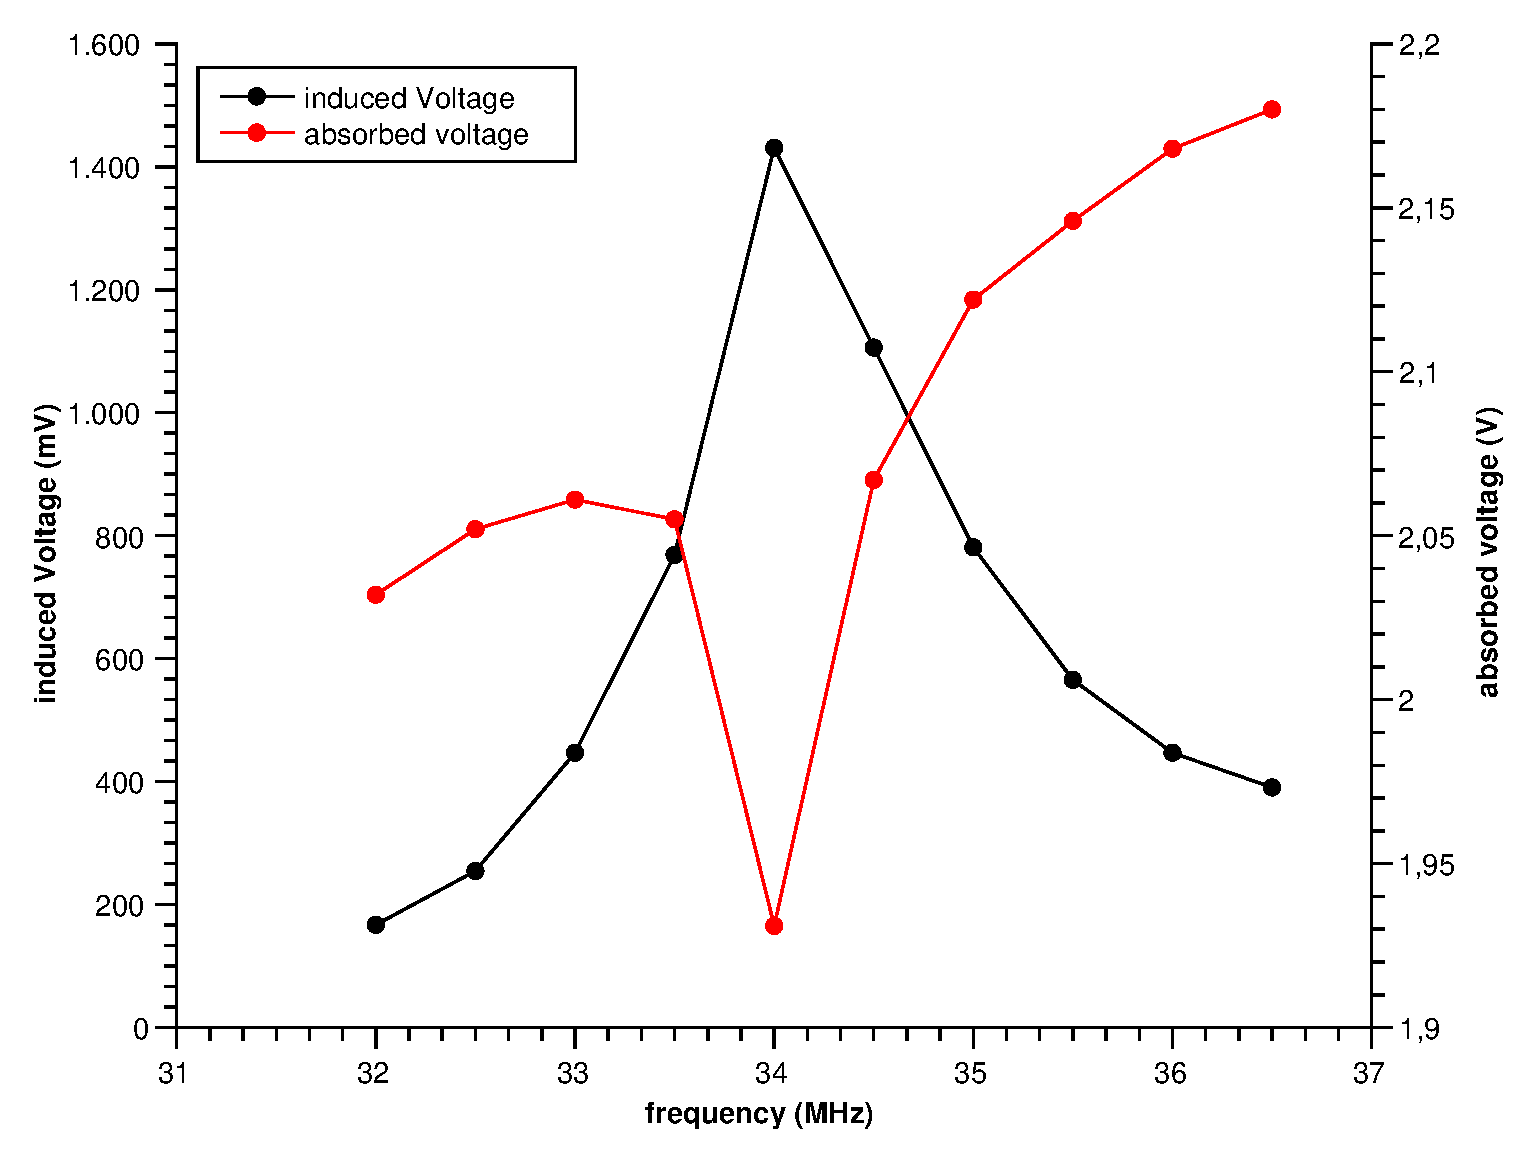
\includegraphics[width=0.8\textwidth]{Capacitor2.eps}
    \caption{Induced and absorbed voltages for capacitor setting 2}
    \label{fig:VoltageCap2}
\end{figure}

\begin{figure}[!ht]
    \centering    
    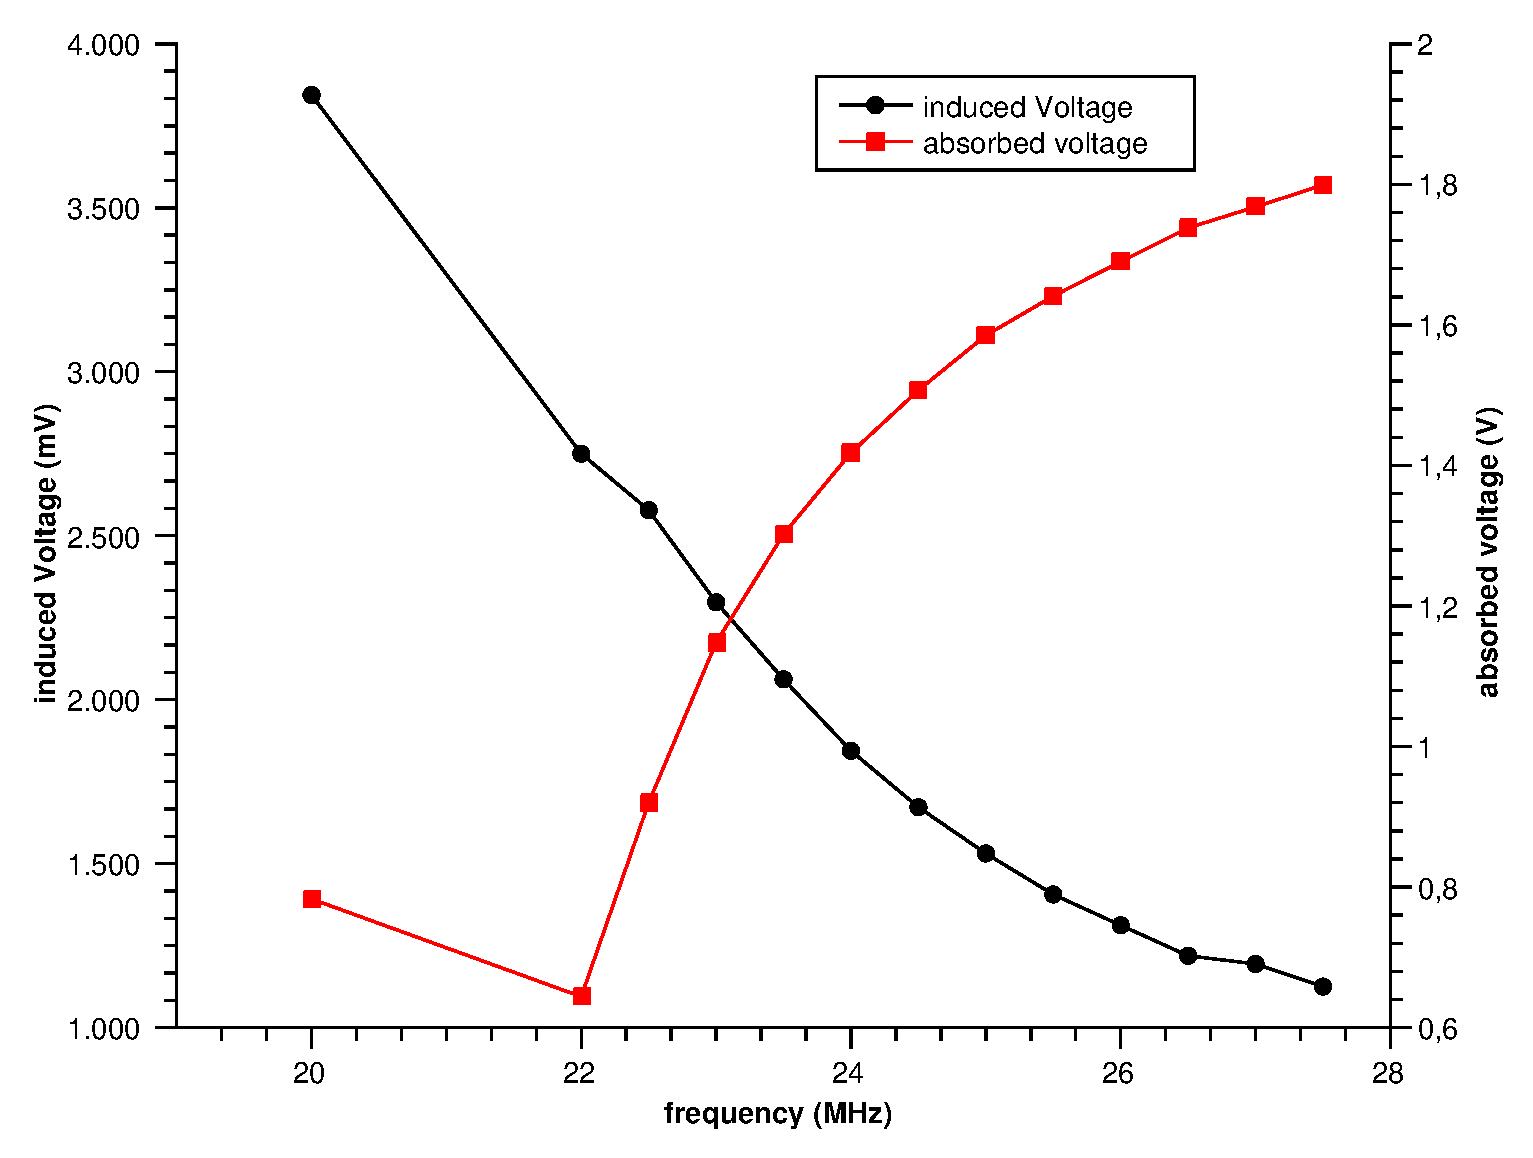
\includegraphics[width=0.8\textwidth]{Capacitor3.eps}
    \caption{Induced and absorbed voltages for capacitor setting 3}
    \label{fig:VoltageCap3}
\end{figure}
\FloatBarrier

The frequency of the peaks also shifts for the different capacity settings, as seen in fig,~\ref{fig:inducedVoltageComparison}. For a lower capacity, the peak shifts to a lower frequency. The same happens for the higher capacity. This indicates there is a capacititties for which the frequency of the peak of induced voltage is maximum.  

\begin{figure}[!ht]
    \centering
    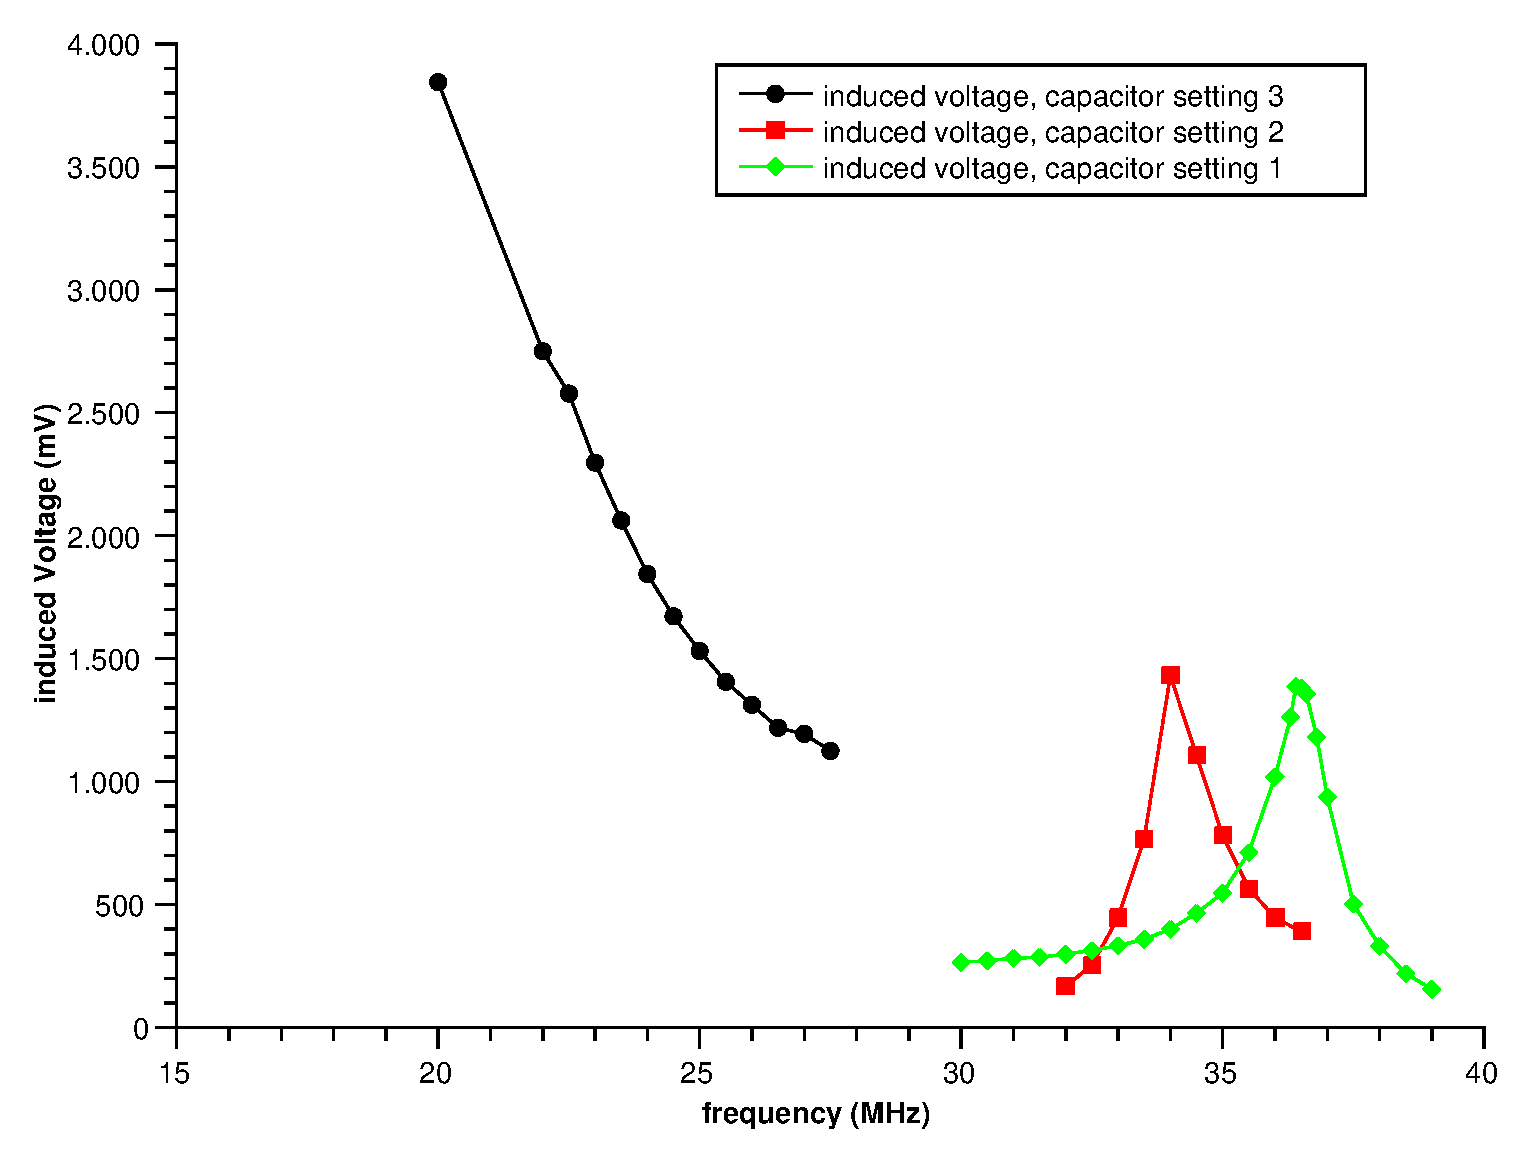
\includegraphics[width=0.8\textwidth]{voltageComparison.eps}
    \caption{Comparison of the induced voltages}
    \label{fig:inducedVoltageComparison}
\end{figure}
\FloatBarrier

\subsection{ESR}
We record the resonance frequency, and plot it as a function of the B-field produced by the Helmholtz coils (which we calculate using eq.~\ref{equation_B}). We obtain a linear relationship as seen in fig.~\ref{fig:f(B)}.

\begin{figure}[!ht]
    \centering
    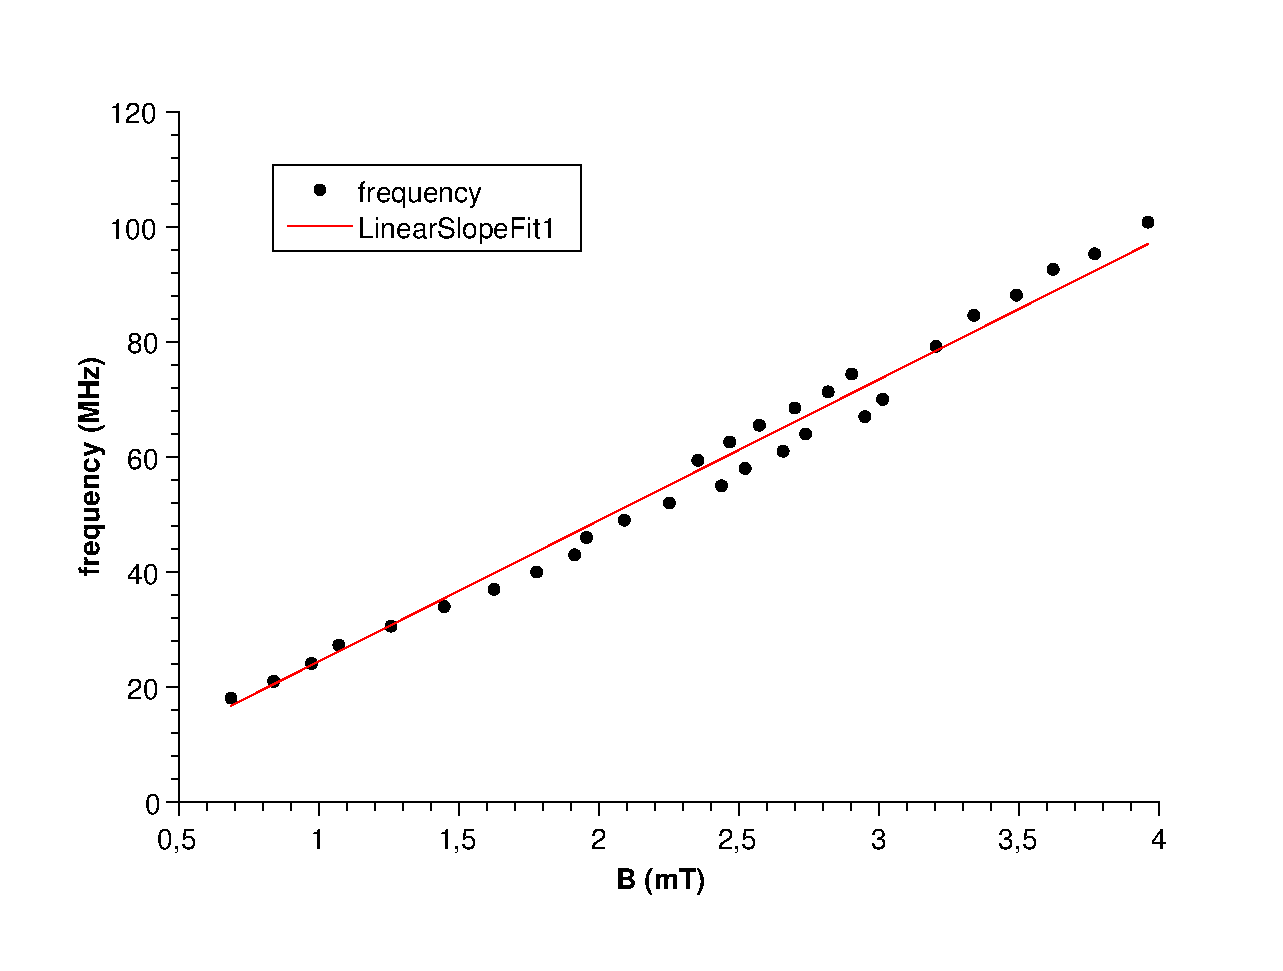
\includegraphics[width=0.8\textwidth]{f_B.eps}
    \caption{Frequency as a function of the magnetic field}
    \label{fig:f(B)}
\end{figure}

The linear fit equation is:
\begin{equation*}
    f = (24.50 \pm 0.21) \cdot B
\end{equation*}

The slope $m$ of the fit is proportional to the Landé factor $g_s$:
\begin{equation*}
    m = \frac{g_s \mu_B}{h}
\end{equation*}

Where $\mu_B = \frac{e \hbar}{2m_e}$ is the Bohr magneton and $h$ is Planck's constant.

This yields:
\begin{align*}
    g_s &= \frac{2m_emh}{e \hbar} \\
    &= \frac{6.626 \cdot 10^{-34} \ \text{J $\cdot$ Hz}^{-1}}{9.274 \cdot 10^{-24} \ \text{J $\cdot$ T}^{-1}} \cdot 24.50 \cdot \frac{10^9}{10^{-3}}\ \text{Hz $\cdot$ T}^{-1} 
\end{align*}

The experimental value of the Landé factor is then:
\begin{equation*}
    \boxed{g_s = 1.75}
\end{equation*}

The theoretical value of the Landé factor is $g_{s,th}$ = 2, so our experimental value deviates by 12.5\% from the theoretical one. 

\section{Conclusion}
In the first part of this lab class, we studied the studied the phenomenon of induced current by magnetic fields. We found that the absorbed and induced voltages where dependent on the frequency of the current generating the magnetic field, and that they reached maxima for the so-called resonance frequency. This frequency was also dependant on the capacity of the other coil.

In the second part we studied electron spin resonance in order to determine the Landé factor. Using the knowledge we gained from the first part, we determined its value to be $g_s = 1.75$, which has a deviation of 12.5~\% from theoretical value.

\end{document}